\documentclass[a4paper]{article}
\usepackage[utf8]{inputenc}
\usepackage[T1]{fontenc}
\usepackage[landscape, top=1.2cm, bottom=1.2cm, left=1.2cm, right=1.2cm]{geometry}
\usepackage{tikz}
\usetikzlibrary{positioning, arrows.meta, calc}

\pagestyle{empty}

% -------------------------------------------------------
% Styles for UML class boxes
% -------------------------------------------------------
\tikzset{
  % Stereotype row  (e.g. <<interface>>)
  ctop/.style={
    draw, fill=white, minimum width=4cm, text centered,
    inner sep=3pt, font=\small\itshape
  },
  % Class name row
  cname/.style={
    draw, fill=white, minimum width=4cm, text centered,
    inner sep=3pt, font=\small\bfseries
  },
  % Attributes / methods row
  cbody/.style={
    draw, fill=white, minimum width=4cm, text width=3.8cm,
    align=left, inner sep=3pt, font=\scriptsize
  },
  % Wider name for ZigZagDown (long attribute names)
  cnamew/.style={
    draw, fill=white, minimum width=5cm, text centered,
    inner sep=3pt, font=\small\bfseries
  },
  % Wider body for ZigZagDown
  cbodyw/.style={
    draw, fill=white, minimum width=5cm, text width=4.8cm,
    align=left, inner sep=3pt, font=\scriptsize
  },
  % Arrow: implementation (dashed, hollow triangle at interface end)
  impl/.style={
    draw, dashed, -{Triangle[open, scale=1.4]},
    shorten >=1pt, shorten <=1pt
  },
  % Arrow: directed association (solid, hollow arrowhead)
  assoc/.style={
    draw, -{Triangle[open, scale=1.4]},
    shorten >=1pt, shorten <=1pt
  },
  % Arrow: dependency (dashed, hollow arrowhead)
  dep/.style={
    draw, dashed, -{Triangle[open, scale=1.4]},
    shorten >=1pt, shorten <=1pt
  }
}

\begin{document}
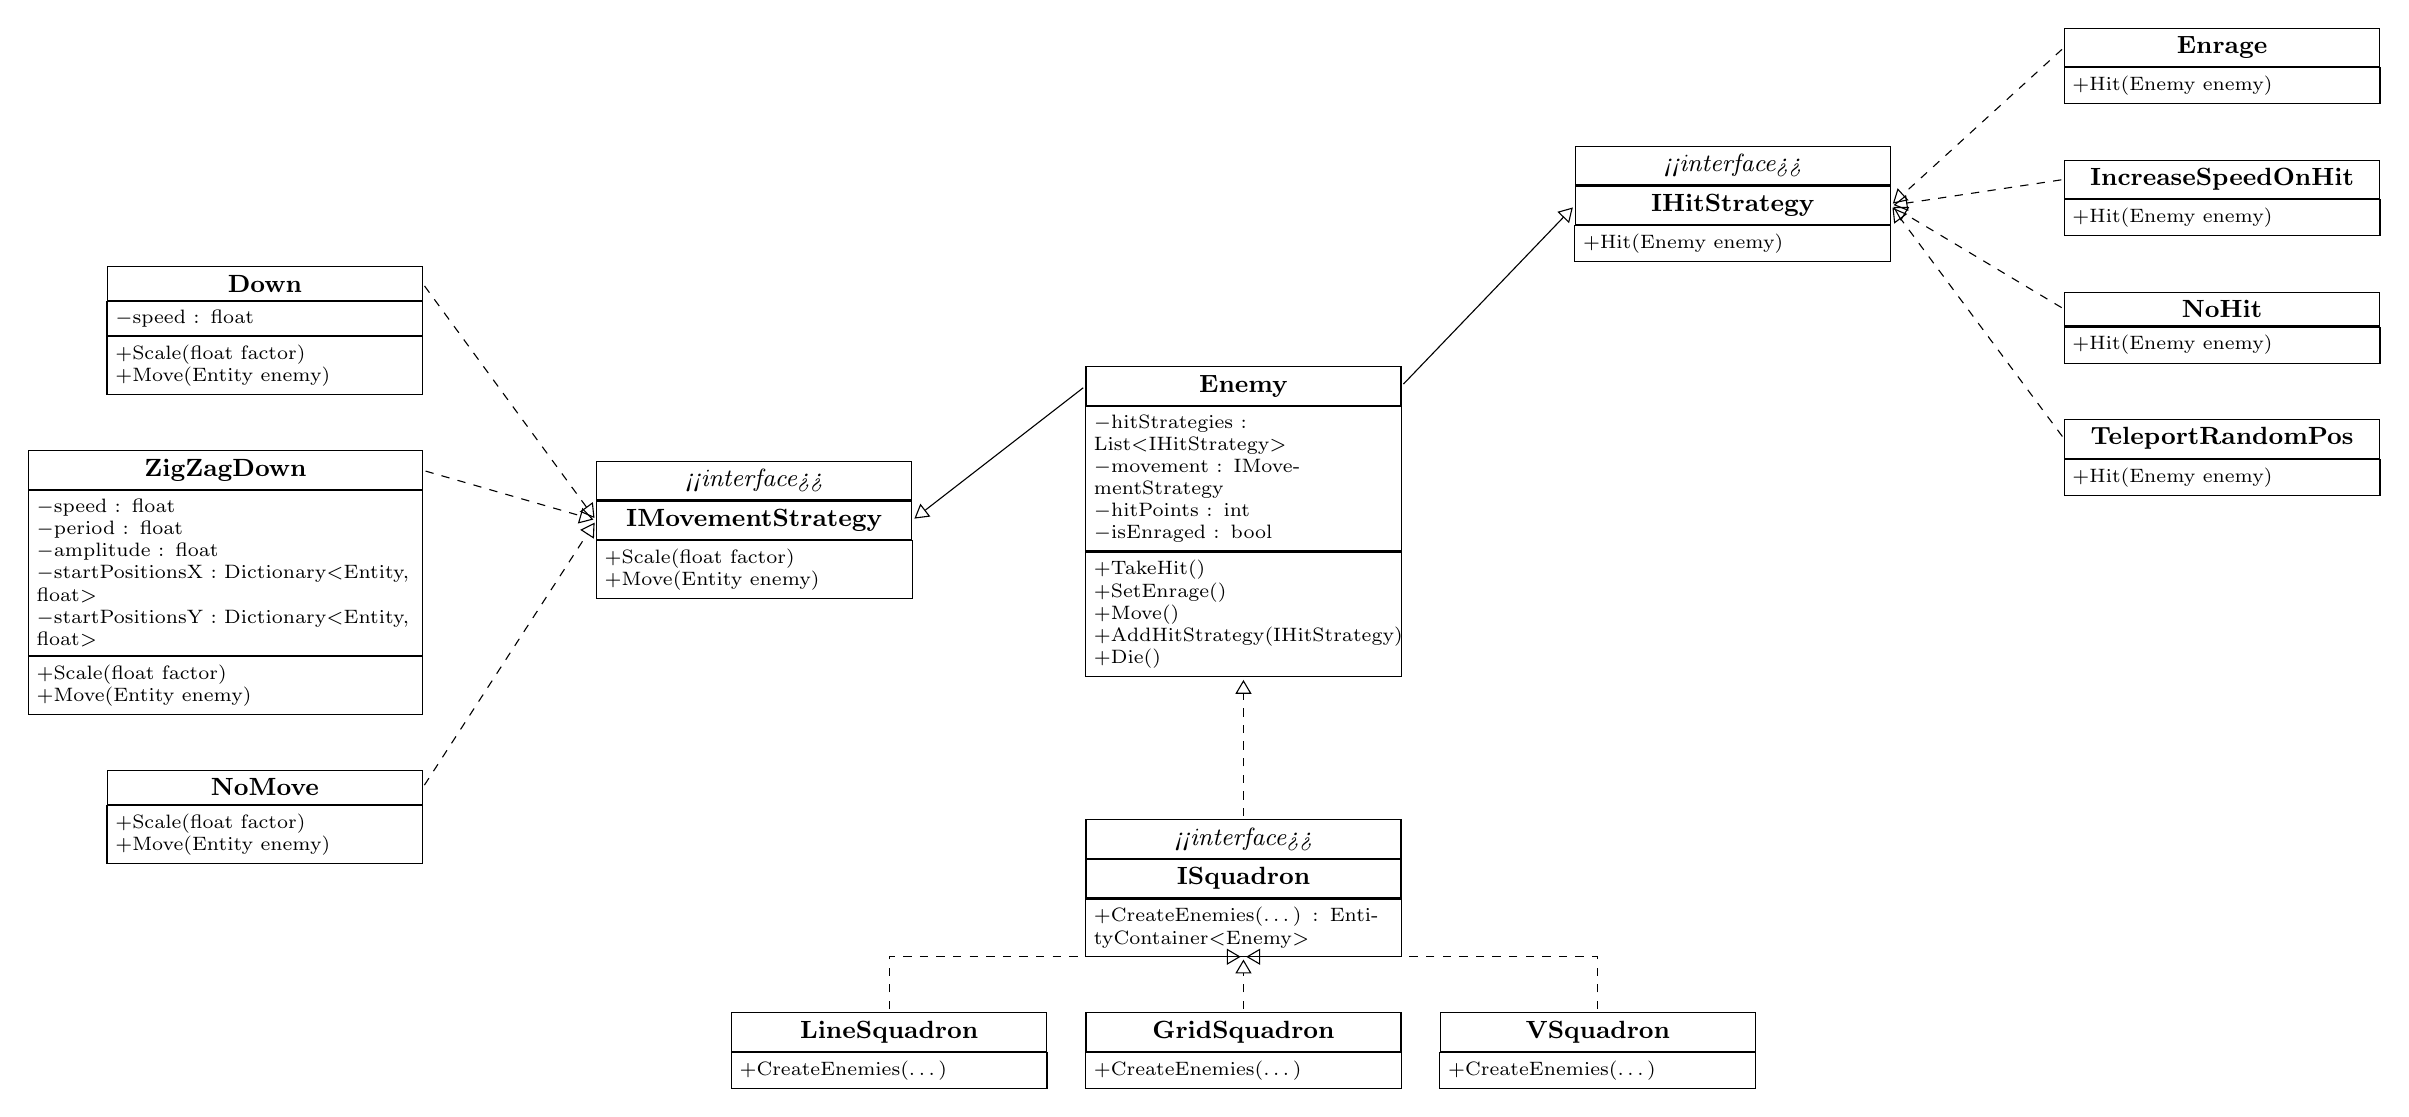
\begin{tikzpicture}[font=\small, node distance=0cm and 0cm]

% ============================================================
% COLUMN 2 -- IMovementStrategy interface (centre-left)
% ============================================================
\node[ctop]  (ims-top)  {<<interface>>};
\node[cname, below=0 of ims-top]  (ims-name) {IMovementStrategy};
\node[cbody, below=0 of ims-name] (ims-body) {
  +Scale(float factor)\\
  +Move(Entity enemy)};

% ============================================================
% COLUMN 1 -- Movement implementations (left of IMS)
% ============================================================

% Down
\node[cname, left=2.2cm of ims-top, yshift=2.5cm] (down-name) {Down};
\node[cbody, below=0 of down-name] (down-attrs) {$-$speed : float};
\node[cbody, below=0 of down-attrs] (down-body) {
  +Scale(float factor)\\
  +Move(Entity enemy)};

% ZigZagDown  (wider box; xshift centres it on the same east-edge as Down)
\node[cnamew, below=0.7cm of down-body, xshift=-0.5cm] (zzd-name) {ZigZagDown};
\node[cbodyw, below=0 of zzd-name] (zzd-attrs) {
  $-$speed : float\\
  $-$period : float\\
  $-$amplitude : float\\
  $-$startPositionsX : Dictionary\textless{}Entity, float\textgreater{}\\
  $-$startPositionsY : Dictionary\textless{}Entity, float\textgreater{}};
\node[cbodyw, below=0 of zzd-attrs] (zzd-body) {
  +Scale(float factor)\\
  +Move(Entity enemy)};

% NoMove  (re-centred to align east-edge with Down and ZigZagDown)
\node[cname, below=0.7cm of zzd-body, xshift=0.5cm] (nomove-name) {NoMove};
\node[cbody, below=0 of nomove-name] (nomove-body) {
  +Scale(float factor)\\
  +Move(Entity enemy)};

% ============================================================
% COLUMN 3 -- Enemy (centre)
% ============================================================
\node[cname, right=2.2cm of ims-top, yshift=1.2cm] (enemy-name) {Enemy};
\node[cbody, below=0 of enemy-name] (enemy-attrs) {
  $-$hitStrategies : List\textless{}IHitStrategy\textgreater{}\\
  $-$movement : IMovementStrategy\\
  $-$hitPoints : int\\
  $-$isEnraged : bool};
\node[cbody, below=0 of enemy-attrs] (enemy-body) {
  +TakeHit()\\
  +SetEnrage()\\
  +Move()\\
  +AddHitStrategy(IHitStrategy)\\
  +Die()};

% ============================================================
% COLUMN 4 -- IHitStrategy interface (centre-right)
% ============================================================
\node[ctop,  right=2.2cm of enemy-name, yshift=2.8cm] (ihs-top)  {<<interface>>};
\node[cname, below=0 of ihs-top]  (ihs-name) {IHitStrategy};
\node[cbody, below=0 of ihs-name] (ihs-body) {+Hit(Enemy enemy)};

% ============================================================
% COLUMN 5 -- Hit-strategy implementations (right of IHS)
% ============================================================

% Enrage
\node[cname, right=2.2cm of ihs-top, yshift=1.5cm] (enrage-name) {Enrage};
\node[cbody, below=0 of enrage-name] (enrage-body) {+Hit(Enemy enemy)};

% IncreaseSpeedOnHit
\node[cname, below=0.7cm of enrage-body] (ish-name) {IncreaseSpeedOnHit};
\node[cbody, below=0 of ish-name] (ish-body) {+Hit(Enemy enemy)};

% NoHit
\node[cname, below=0.7cm of ish-body] (nohit-name) {NoHit};
\node[cbody, below=0 of nohit-name] (nohit-body) {+Hit(Enemy enemy)};

% TeleportRandomPos
\node[cname, below=0.7cm of nohit-body] (trp-name) {TeleportRandomPos};
\node[cbody, below=0 of trp-name] (trp-body) {+Hit(Enemy enemy)};

% ============================================================
% ISquadron + implementations (below Enemy)
% ============================================================
\node[ctop,  below=1.8cm of enemy-body] (isq-top)  {<<interface>>};
\node[cname, below=0 of isq-top]  (isq-name) {ISquadron};
\node[cbody, below=0 of isq-name] (isq-body) {
  +CreateEnemies(\dots) : EntityContainer\textless{}Enemy\textgreater{}};

% LineSquadron
\node[cname, below=0.7cm of isq-body, xshift=-4.5cm] (ls-name) {LineSquadron};
\node[cbody, below=0 of ls-name] (ls-body) {+CreateEnemies(\dots)};

% GridSquadron (directly below ISquadron)
\node[cname, below=0.7cm of isq-body] (gs-name) {GridSquadron};
\node[cbody, below=0 of gs-name] (gs-body) {+CreateEnemies(\dots)};

% VSquadron
\node[cname, below=0.7cm of isq-body, xshift=4.5cm] (vs-name) {VSquadron};
\node[cbody, below=0 of vs-name] (vs-body) {+CreateEnemies(\dots)};

% ============================================================
% ARROWS
% ============================================================

% -- Movement implementations --implements--> IMovementStrategy --
% Diagonal lines fan into ims-name.west (the class-name section).
\draw[impl] (down-name.east)   -- (ims-name.west);
\draw[impl] (zzd-name.east)    -- (ims-name.west);
\draw[impl] (nomove-name.east) -- (ims-name.west);

% -- Enemy --uses--> IMovementStrategy  (directed association) --
\draw[assoc] (enemy-name.west) -- (ims-name.east);

% -- Enemy --uses--> IHitStrategy  (directed association) --
\draw[assoc] (enemy-name.east) -- (ihs-name.west);

% -- Hit implementations --implements--> IHitStrategy --
% Diagonal lines fan into ihs-name.east (the class-name section).
\draw[impl] (enrage-name.west) -- (ihs-name.east);
\draw[impl] (ish-name.west)    -- (ihs-name.east);
\draw[impl] (nohit-name.west)  -- (ihs-name.east);
\draw[impl] (trp-name.west)    -- (ihs-name.east);

% -- ISquadron --depends--> Enemy --
\draw[dep] (isq-top.north) -- (enemy-body.south);

% -- Squadron implementations --implements--> ISquadron --
% ls and vs use elbow routing; gs goes straight up.
\draw[impl] (ls-name.north) |- (isq-body.south);
\draw[impl] (gs-name.north) -- (isq-body.south);
\draw[impl] (vs-name.north) |- (isq-body.south);

\end{tikzpicture}
\end{document}
